%%% Local Variables:
%%% mode: latex
%%% TeX-master: "../index"
%%% End:

% Recommended:
% Show symmetric-key example with Alice-Bob diagram
% Mention modern algorithm (e.g. AES, Triple-DES)
% Benefits of public-key encryption (no key sharing)
% Show public-key example with RSA and Alice-Bob diagram

\subsection*{Agenda}
\begin{enumerate}
\item Symmetric-key encryption
\item Symmetric- vs. public-key encryption
\item Public-key encryption
\item RSA
\end{enumerate}

\subsection{Symmetric-key encryption}
\subsubsection*{Set up}
\begin{itemize}
\item $m \in \mathcal{P}$ is the plaintext
\item $k \in \mathcal{K}$ is the key
\item $c \in \mathcal{C}$ is the ciphertext
\item $e_k(m)$ encryption function
\item $d_k(c)$ decryption function
\end{itemize}

\begin{figure}[H]
  \begin{centering}
    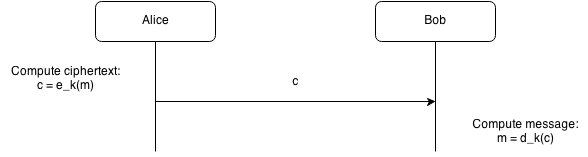
\includegraphics[width=15cm]{images/1-sym-enc}
    \caption{Basic model for symmetric encryption}
  \end{centering}
  \label{fig:sym-enc}
\end{figure}

\subsubsection*{Modern implementations}
\begin{description}
\item[DES] 64-bit block cipher with 56-bit key. Due to small key,
  exhaustive search is a possibility. Therefore, \emph{Triple-DES} was
  made.
\item[AES] 128-bit block cipher with 128 to 256-bit key.
\end{description}

\subsection{Symmetric- vs. public-key encryption}
\begin{description}
\item[Pros] Faster and easier to implement
\item[Cons] Requires both parties can access the secret key. Impossible?
\end{description}

\subsection{Public-key encryption}
\begin{figure}[H]
  \begin{centering}
    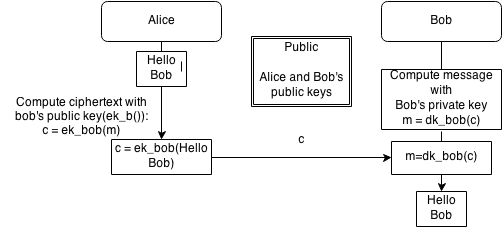
\includegraphics[width=15cm]{images/1-pub-enc}
    \caption{Basic model for public encryption}
  \end{centering}
  \label{fig:pub-enc}
\end{figure}

\subsection{RSA}

%%% Local Variables: 
%%% mode: latex
%%% TeX-master: "../index"
%%% End: 
\subsection*{Setup}
\textbf{Public key:} $(n, e)$ where $n = pq$ for primes $p, q$ and $e \in \mathbb{Z}_{\phi(n)}^*$

\textbf{Private key:} $(p, q, d)$ where $d \in \mathbb{Z}_{\phi(n)}^*$, such that
\[ ed \equiv 1 \mod \phi(n) \]

We use $\phi(n)$ because it is hard to compute given only a large $n$, but easy with known $p, q$ since $\phi(n) = (p-1)(q-1)$, thus $d$ cannot be easily computed given just $n$ (must prime factor $n$).

\textbf{Encryption:} $m$ is the message. Encryption is
\[ Enc(m) = m^e \mod n \]

\textbf{Decryption:} $c$ is the ciphertext. Decryption is as follows:
\[ Dec(c) \equiv c^d \mod n \]
\[ Dec(c) \equiv m^{ed} \mod n \]

\textbf{Properties of RSA:}

$e$ must be chosen such that it holds that $gcd(\phi(n),e) = 1$, where
$\phi(n) = (p - 1)(q - 1)$

$n$ must be the product of two large primes $p$ and $q$.


\subsubsection*{Weaknesses of RSA}
%%% Local Variables:
%%% mode: latex
%%% TeX-master: "../index"
%%% End:

\begin{itemize}
\item If attacker can factor $n$ then he can find $d$ same way that
    the system computes it
\item Attacker finds $\phi (n)$, then he can compute $d$ and find factors of $n$ and thereby break the system.
  \begin{itemize}
  \item If $n$ is small attacker can setup an equation with two unknowns
    that uses $\phi (n)=(p-1)(q-1)$ since he knows $n=pq$
    \begin{align*}
      \phi(n) &= n - p - q + 1 \\
      p &= n - \phi(n) - q + 1 \quad \text{since } p = \frac{n}{q} \\
      \frac{n}{q} &= n - \phi(n) - q + 1 \\
      0 &= q^2 + q(\phi(n) - n - 1) + n
    \end{align*}
  \end{itemize}
\item Attacker finds the decryption exponent $d$, factors $n$ and breaks the system
\end{itemize}

\subsubsection*{Proof}
%%% Local Variables:
%%% mode: latex
%%% TeX-master: "../index"
%%% End:

\textbf{Public:} $n = pq$ for primes $p, q$ and encryption exponent $e
\in \mathbb{Z}_{\phi(n)}^*$

\textbf{Private:} $(p, q, d)$ where $d \in \mathbb{Z}_{\phi(n)}^*$, such that
\[ ed \equiv 1 \mod \phi(n) \]

Define $\phi(n) = (p-1)(q-1)$. We have that
\begin{align*}
  & ed \equiv 1 \mod \phi(n)\\
  \Rightarrow\quad& ed = 1 + k(p - 1)(q - 1) \quad \text{where } k \in \mathbb{Z}
\end{align*}

We need to prove that $(m^e)^d \equiv m \mod$ since that is enc and dec using RSA.
\begin{align*}
(m^e)^d &\equiv m \mod n \\
\Rightarrow\quad m^{ed} &\equiv m \mod n
\end{align*}

Chinese Remainder Theorem says that it is enough to show
\[ m^{ed} \equiv m \mod p \quad \textbf{and} \quad m^{ed} \equiv m \mod q \]

Showing for $p$. There are two cases: 1) $m \equiv 0 \mod p$ and 2) $m \not\equiv 0 \mod p$.

\textbf{Case 1}
\begin{align*}
  m &\equiv 0 \mod p\\
  \Rightarrow\quad m^x &\equiv m \mod p \quad \text{for } x \in \mathbb{Z}
\end{align*}
Since $ed \in \mathbb{Z}$, case 1 holds.

\textbf{Case 2}
\begin{align*}
m &\equiv m^{ed} \mod p \\
  &\equiv m^{1 + k(p-1)(q-1)} \mod p \\
  &\equiv m \cdot m^{k(p-1)(q-1)} \mod p \\
  &\equiv m \cdot (m^{(p-1)})^{k(q-1)} \mod p
\end{align*}

From Fermat's little theorem (\ref{sec:fermats-little}) we know that
$x^{p-1} \equiv x \mod p$ for prime $p$. Thus
\begin{align*}
m &\equiv m \cdot 1^{k(q-1)} \mod p \\
  &\equiv m \cdot 1 \mod p \\
  &\equiv m \mod p
\end{align*}

Therefore, case 2 also holds and we have proved for prime $p$.

